This chapter presents the design of a safe controller for the  robotic patient manipulator with a fixed region defined as the unsafe region. Only the controllable part of the robotic patient manipulator is considered, meaning the joints in the robot "hand" and instrument, as displayed in \autoref{fig:robot_hand_unsafe_region}. The controller is designed for and tested on the da Vinci robot comprising the prismatic slide joint as described in \autoref{chap:cbf_1d_static} as well as five independent revolute joints.

\begin{figure}[htbp]
\centering
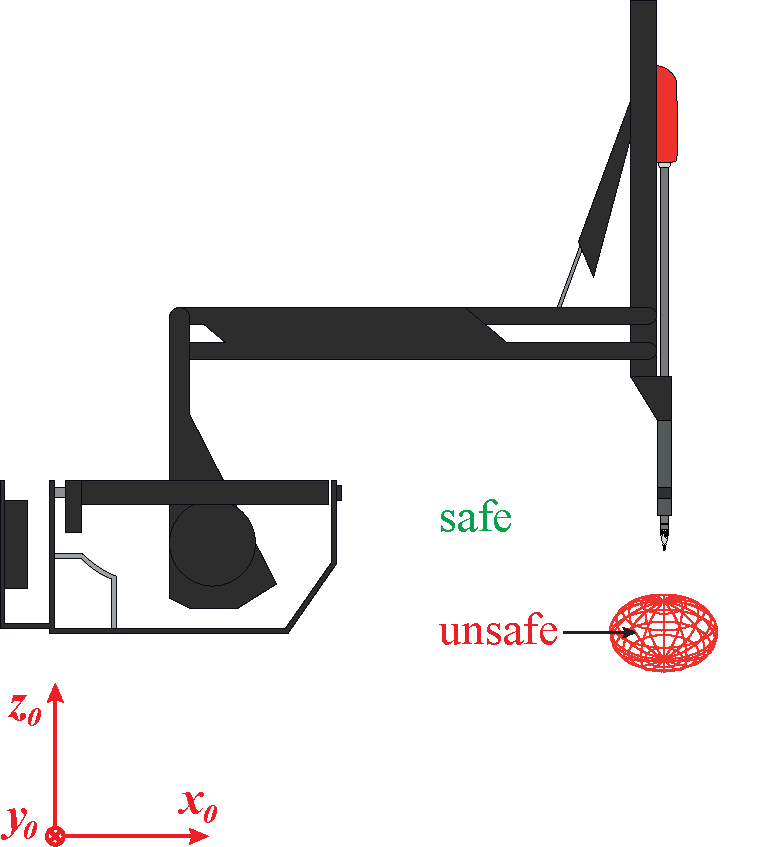
\includegraphics[width=0.45\textwidth]{robot_hand_unsafe_region.pdf}
\caption{Robotic patient manipulator "hand" and instrument, i.e. the controllable parts of the patient manipulator, and a fixed region within the reachable space $\mathcal{X}$ that is unsafe, $\mathcal{X}_u$, marked by a red ellipsoid. INCLUDE ILLUSTRATION FROM RVIZ!}
\label{fig:robot_hand_unsafe_region}
\end{figure}

Introduce that in order to design a controller first kinematics for the robot is defined in order that we can make this a controller in a Cartesian state-space and not in the joint state-space.

(for a thorough kinematic description of the AAU da Vinci robot see \autoref{app:kinematic_model_robot})

\section{Defining the Kinematics of the AAU da Vinci Robot}
KINEMATICS: from appendix, introduce frames for each joint, rotation and translation constitutes transformation matrix between frames, summary of what is in appendix C first page. Explain about DH and the difference to the way kinematic transformation is defined in xacro incl code snip. Include figure C4b ad last part of table C7 and mark the mimick joints (maybe also have to include figure C1b and last par of table C1?)

\subsection{Employing Inverse Kinematics for a Controller in 3D Cartesian Space}
The controller is developed for 3D position and orientation control of the tool tip, and relies on the \gls{kdl} inverse kinematics solver to map from the desired 3D Cartesian space configuration to a prudent 6D joint space position of the da Vinci robotic patient manipulator, in order to pass the transformed joint position commands to the low level controllers (see \autoref{fig:overview}).

The \gls{ik} \gls{kdl} solver employed in \gls{ros} relies on the kinematic chain from the URDF, which is generated from the \texttt{xacro} link and joint kinematic description as presented in %\autoref{app:kinematic_model_robot}, the model implemented in ROS defined in
\autoref{sec:app_activejoints_kinematics}. From this chain (\texttt{my\_chain} in the below example) a \gls{fk} position solver is created along with an \gls{ik} velocity solver in order to define the \gls{ik} position solver:

\begin{lstlisting}[language=xml]
//Create solver based on kinematic chain
KDL::ChainFkSolverPos_recursive fksolver(my_chain);
KDL::ChainIkSolverVel_pinv iksolverv(my_chain);
KDL::ChainIkSolverPos_NR iksolver = KDL::ChainIkSolverPos_NR(my_chain,fksolver,iksolverv,100,1e-6);

KDL::JntArray q(my_chain.getNrOfJoints());
KDL::JntArray q_init(my_chain.getNrOfJoints());

//Set destination frame
double x, y, z;
std::cout << "Set end-effector position <x y z>:" << std::endl;
std::cin >> x >> y >> z;
KDL::Vector dest_pos(x,y,z);
KDL::Frame dest_frame(dest_pos);

// Compute!
int ret = iksolver.CartToJnt(q_init,dest_frame,q);
\end{lstlisting}

The \gls{kdl} \gls{ik} position solver uses the Newton-Raphson iterative numerical technique through the function \texttt{CartToJnt} to determine a prudent joint configuration implementing the desired Cartesian configuration (given as \texttt{dest\_frame} in the above example). In the above example the initial guess \texttt{q\_init} of the joint configuration is the current joint configuration, and hence care should be taken to only command small changes in configuration for the sake of fast convergence of the \gls{ik} solution.


Three dimensional positions of the tool tip is described in a frame oriented as the inertial frame and offset such that a robot configuration with all free angles and slide set to zero equals a position of the tool tip in [0,0,0].
The ellipsoid enclosing the region $\mathcal{X}_u$ in \autoref{fig:robot_hand_unsafe_region} is defined as the zero level set of a function of the form:
\begin{equation}
B(x,y,z) = -\left(  \left(\frac{x-c_x}{r_x}\right)^2 + \left(\frac{y-c_y}{r_y}\right)^2 + \left(\frac{z-c_z}{r_z}\right)^2 - 1 \right)
\end{equation}
\begin{tabular}{rl}
where&\\
$[c_x\,\, c_y\,\, c_z]$ & is the coordinate of the center of the ellipsoid\\
$[r_x\,\, r_y\,\, r_z]$ & is the length of the semi-axes of the ellipsoid\\
\end{tabular}


\section{Modelling of Robot Hand Movement}
\textcolor{red}{Make measurement of step for cases: x-axis, y-axis, z-axis, and xyz at the same time.}

\section{Safe Controller Design for First Order System}

A decoupled first order system is assumed for each of the three axes on the form

\begin{equation}
\small
\dot{\begin{bmatrix}
	x\\y\\z
	\end{bmatrix}} =
\begin{bmatrix}
-1/\tau & 0 & 0\\0 & -1/\tau & 0 \\ 0 & 0 & -1/\tau
\end{bmatrix}
\begin{bmatrix}
x\\y\\z
\end{bmatrix} +
\begin{bmatrix}
1/\tau& 0 & 0 \\ 0& 1/\tau & 0 \\0& 0& 1/\tau
\end{bmatrix} 
\left(
\begin{bmatrix}
\bar{N} & 0 & 0 \\0 & \bar{N} & 0 \\0& 0& \bar{N}
\end{bmatrix}
\begin{bmatrix}
x_{ref}\\y_{ref}\\z_{ref}
\end{bmatrix}
-
\begin{bmatrix}
k_x & 0 & 0 \\0 & k_y & 0 \\0& 0&  k_z
\end{bmatrix}
\begin{bmatrix}
x\\y\\z
\end{bmatrix}
\right)
\end{equation}

\textcolor{green}{Giver modellen mening?}

\section{Safe Controller Design for Second Order System}